%%%%%%%%%%%%%%%%%%%%%%%%%%%%%%%%%%%%%%%%%
% Arsclassica Article
% LaTeX Template
% Version 1.1 (10/6/14)
%
% This template has been downloaded from:
% http://www.LaTeXTemplates.com
%
% Original author:
% Lorenzo Pantieri (http://www.lorenzopantieri.net) with extensive modifications by:
% Vel (vel@latextemplates.com)
%
% License:
% CC BY-NC-SA 3.0 (http://creativecommons.org/licenses/by-nc-sa/3.0/)
%
%%%%%%%%%%%%%%%%%%%%%%%%%%%%%%%%%%%%%%%%%

%----------------------------------------------------------------------------------------
%	PACKAGES AND OTHER DOCUMENT CONFIGURATIONS
%----------------------------------------------------------------------------------------

\documentclass[
10pt, % Main document font size
letterpaper, % Paper type, use 'letterpaper' for US Letter paper
oneside, % One page layout (no page indentation)
%twoside, % Two page layout (page indentation for binding and different headers)
headinclude,footinclude, % Extra spacing for the header and footer
BCOR5mm, % Binding correction
]{scrartcl}

%%%%%%%%%%%%%%%%%%%%%%%%%%%%%%%%%%%%%%%%%
% Arsclassica Article
% Structure Specification File
%
% This file has been downloaded from:
% http://www.LaTeXTemplates.com
%
% Original author:
% Lorenzo Pantieri (http://www.lorenzopantieri.net) with extensive modifications by:
% Vel (vel@latextemplates.com)
%
% License:
% CC BY-NC-SA 3.0 (http://creativecommons.org/licenses/by-nc-sa/3.0/)
%
%%%%%%%%%%%%%%%%%%%%%%%%%%%%%%%%%%%%%%%%%

%----------------------------------------------------------------------------------------
%	REQUIRED PACKAGES
%----------------------------------------------------------------------------------------

\usepackage[
nochapters, % Turn off chapters since this is an article        
beramono, % Use the Bera Mono font for monospaced text (\texttt)
eulermath,% Use the Euler font for mathematics
pdfspacing, % Makes use of pdftex’ letter spacing capabilities via the microtype package
dottedtoc % Dotted lines leading to the page numbers in the table of contents
]{classicthesis} % The layout is based on the Classic Thesis style

\usepackage{arsclassica} % Modifies the Classic Thesis package

\usepackage[T1]{fontenc} % Use 8-bit encoding that has 256 glyphs

\usepackage[utf8]{inputenc} % Required for including letters with accents

\usepackage{graphicx} % Required for including images
\graphicspath{{Figures/}} % Set the default folder for images

\usepackage{enumitem} % Required for manipulating the whitespace between and within lists

\usepackage{lipsum} % Used for inserting dummy 'Lorem ipsum' text into the template

\usepackage{subfig} % Required for creating figures with multiple parts (subfigures)

\usepackage{amsmath,amssymb,amsthm} % For including math equations, theorems, symbols, etc

\usepackage{varioref} % More descriptive referencing

\usepackage{url}

\usepackage{listings}

\usepackage[numbers]{natbib} % required for cite author to work
%----------------------------------------------------------------------------------------
%	THEOREM STYLES
%---------------------------------------------------------------------------------------

\theoremstyle{definition} % Define theorem styles here based on the definition style (used for definitions and examples)
\newtheorem{definition}{Definition}

\theoremstyle{plain} % Define theorem styles here based on the plain style (used for theorems, lemmas, propositions)
\newtheorem{theorem}{Theorem}

\theoremstyle{remark} % Define theorem styles here based on the remark style (used for remarks and notes)

%----------------------------------------------------------------------------------------
%	HYPERLINKS
%---------------------------------------------------------------------------------------

\hypersetup{
%draft, % Uncomment to remove all links (useful for printing in black and white)
colorlinks=true, breaklinks=true, bookmarks=true,bookmarksnumbered,
urlcolor=webbrown, linkcolor=RoyalBlue, citecolor=webgreen, % Link colors
pdftitle={}, % PDF title
pdfauthor={\textcopyright}, % PDF Author
pdfsubject={}, % PDF Subject
pdfkeywords={}, % PDF Keywords
pdfcreator={pdfLaTeX}, % PDF Creator
pdfproducer={LaTeX with hyperref and ClassicThesis} % PDF producer
}

%----------------------------------------------------------------------------------------
%	REnew commands
%---------------------------------------------------------------------------------------
\newcommand{\breakrule}{
\begin{center}
\noindent\rule{8cm}{0.4pt}
\end{center}
}

%----------------------------------------------------------------------------------------
%	Code listing
%---------------------------------------------------------------------------------------
\usepackage{listings}
\usepackage{color}
 
\definecolor{codegreen}{rgb}{0,0.6,0}
\definecolor{codegray}{rgb}{0.5,0.5,0.5}
\definecolor{codepurple}{rgb}{0.58,0,0.82}
\definecolor{backcolour}{rgb}{0.95,0.95,0.92}

\lstdefinestyle{mystyle}{
    backgroundcolor=\color{backcolour},   
    commentstyle=\color{codegreen},
    keywordstyle=\color{magenta},
    numberstyle=\tiny\color{codegray},
    stringstyle=\color{codepurple},
    basicstyle=\footnotesize,
    breakatwhitespace=false,         
    breaklines=true,                 
    captionpos=b,                    
    keepspaces=true,                 
    numbers=left,                    
    numbersep=5pt,                  
    showspaces=false,                
    showstringspaces=false,
    showtabs=false,                  
    tabsize=2
}
 
\lstset{style=mystyle}

\renewcommand{\lstlistingname}{Algorithm}% Listing -> Algorithm
\renewcommand{\lstlistlistingname}{List of \lstlistingname s}% List of Listings -> List of Algorithms

% Quotes

\newenvironment{shadequote}{%
  \begin{center}%
    \begin{minipage}{.8\linewidth}%
      \begin{shaded}%
        \sffamily\slshape}{%
      \end{shaded}
    \end{minipage}%
  \end{center}%
}
\usepackage{framed}
\definecolor{shadecolor}{gray}{0.95}

% adjust for 1 inch margins
% Comment next line for proper behavior!
\usepackage[margin=1in]{geometry}

 % Include the structure.tex file which specified the document structure and layout

\hyphenation{Fortran hy-phen-ation} % Specify custom hyphenation points in words with dashes where you would like hyphenation to occur, or alternatively, don't put any dashes in a word to stop hyphenation altogether

%----------------------------------------------------------------------------------------
%	TITLE AND AUTHOR(S)
%----------------------------------------------------------------------------------------

\title{\normalfont\spacedallcaps{NASA's 2019-2020 MNSGC Intercollegiate Quadcopter Challenge}
    \\Preliminary Design Review} % The article title

\author{Written By: Mikele Finn, Robert Edman,\\
    Tonia Edman, Miranda Larson, \\
    Kenneth Cloud, Devin Wells \\
    Advisor: Eric Kuha \\
    \spacedlowsmallcaps{Institution: Leech Lake Tribal College}} % The article author(s) - author affiliations need to be specified in the AUTHOR AFFILIATIONS block

\date{} % An optional date to appear under the author(s)

%----------------------------------------------------------------------------------------

\begin{document}

%----------------------------------------------------------------------------------------
%	HEADERS
%----------------------------------------------------------------------------------------

\renewcommand{\sectionmark}[1]{\markright{\spacedlowsmallcaps{#1}}} % The header for all pages (oneside) or for even pages (twoside)
%\renewcommand{\subsectionmark}[1]{\markright{\thesubsection~#1}} % Uncomment when using the twoside option - this modifies the header on odd pages
\lehead{\mbox{\llap{\small\thepage\kern1em\color{halfgray} \vline}\color{halfgray}\hspace{0.5em}\rightmark\hfil}} % The header style

\pagestyle{scrheadings} % Enable the headers specified in this block

%----------------------------------------------------------------------------------------
%	TABLE OF CONTENTS & LISTS OF FIGURES AND TABLES
%----------------------------------------------------------------------------------------

\maketitle % Print the title/author/date block

\begin{figure}[!htbp]
    \centering
    
\includegraphics[width=0.4\textwidth]{figs/lltc_logo.png} % first figure itself
    \hfill
    
\includegraphics[width=0.4\textwidth]{figs/stem_logo.png} % second figure itself
\end{figure}

\setcounter{tocdepth}{2} % Set the depth of the table of contents to show sections and subsections only

%----------------------------------------------------------------------------------------
%	AUTHOR AFFILIATIONS
%----------------------------------------------------------------------------------------

% {\let\thefootnote\relax\footnotetext{\textsuperscript{1} \textit{Department of Electrical and Computer Engineering, Northeastern University, Boston, United States}}}

%----------------------------------------------------------------------------------------

\newpage
\tableofcontents % Print the table of contents

\listoffigures % Print the list of figures

% \listoftables % Print the list of tables

%----------------------------------------------------------------------------------------
%	ABSTRACT
%----------------------------------------------------------------------------------------

%\section*{Abstract} % This section will not appear in the table of contents due to the star (\section*)
%TODOOOOOOO
%My Abstract here



\newpage % Start the article content on the second page, remove this if you have a longer abstract that goes onto the second page

% ========================================================================================
%	Question 1
% ========================================================================================

\section{Introduction}

\subsection{The Team}
\begin{itemize}
    \item \textbf{Mikele Finn} - Team Lead - Business Administration major with managerial experience. Team lead and main spokesperson. Pilot
    \item \textbf{Robert Edman} - Elder Statesman -- Lots of experience with problem solving and mechanical expertise.
    \item \textbf{Tonia Edman} - STEM Major, Activites Coordinator -- Procurement and budgeting, Engineering.
    \item \textbf{Miranda Larson} - Law Enforcement and Forestry Major -- Construction, design, and programming.
    \item \textbf{Kenneth Cloud} - Carpentry Major -- With a background in programming and computer knowledge, our primary arduino guru.
    \item \textbf{Devin Wells} - Forestry Major -- Programming and Design.
\end{itemize}


\subsection{Drone Design Philosophy}

Our design philosophy is one of flexibility. We would like our drone to be as flexible and versatile as possible, within the specifications of this kit. As a large, heavy drone, this machine lacks the maneuverability of traditional racing drones. What it lacks in maneuverability, it makes up for in power, longevity, and hauling power. We plan to include a full instrument package, sampling apparatus, and imaging array (either one or two full video cameras).

The instrument package will contain proximity and distance sensors, gyroscope, hall effect sensors, temperature, humidity, and, of course, lights and cameras.

Our sampling apparatus will be designed to retrieve samples of both solids and liquids. A vial, a scoop, and possibly a grabbing arm.

\section{Progress}

\subsection{Blue Heron}

Two students have practiced flying the Blue Heron, though much work remains to be done in this area. We still have not selected our pilot. The plan will be for everyone to practice as much as possible doing some precision flying of the Blue Heron and whoever is most comfortable with it, will graduate to <Need Name>. All students are expected to be passably competent so we have backups in case of illness on the day of the event.

\subsection{Flame Wheel}

\begin{figure}[!htbp]
\centering 
        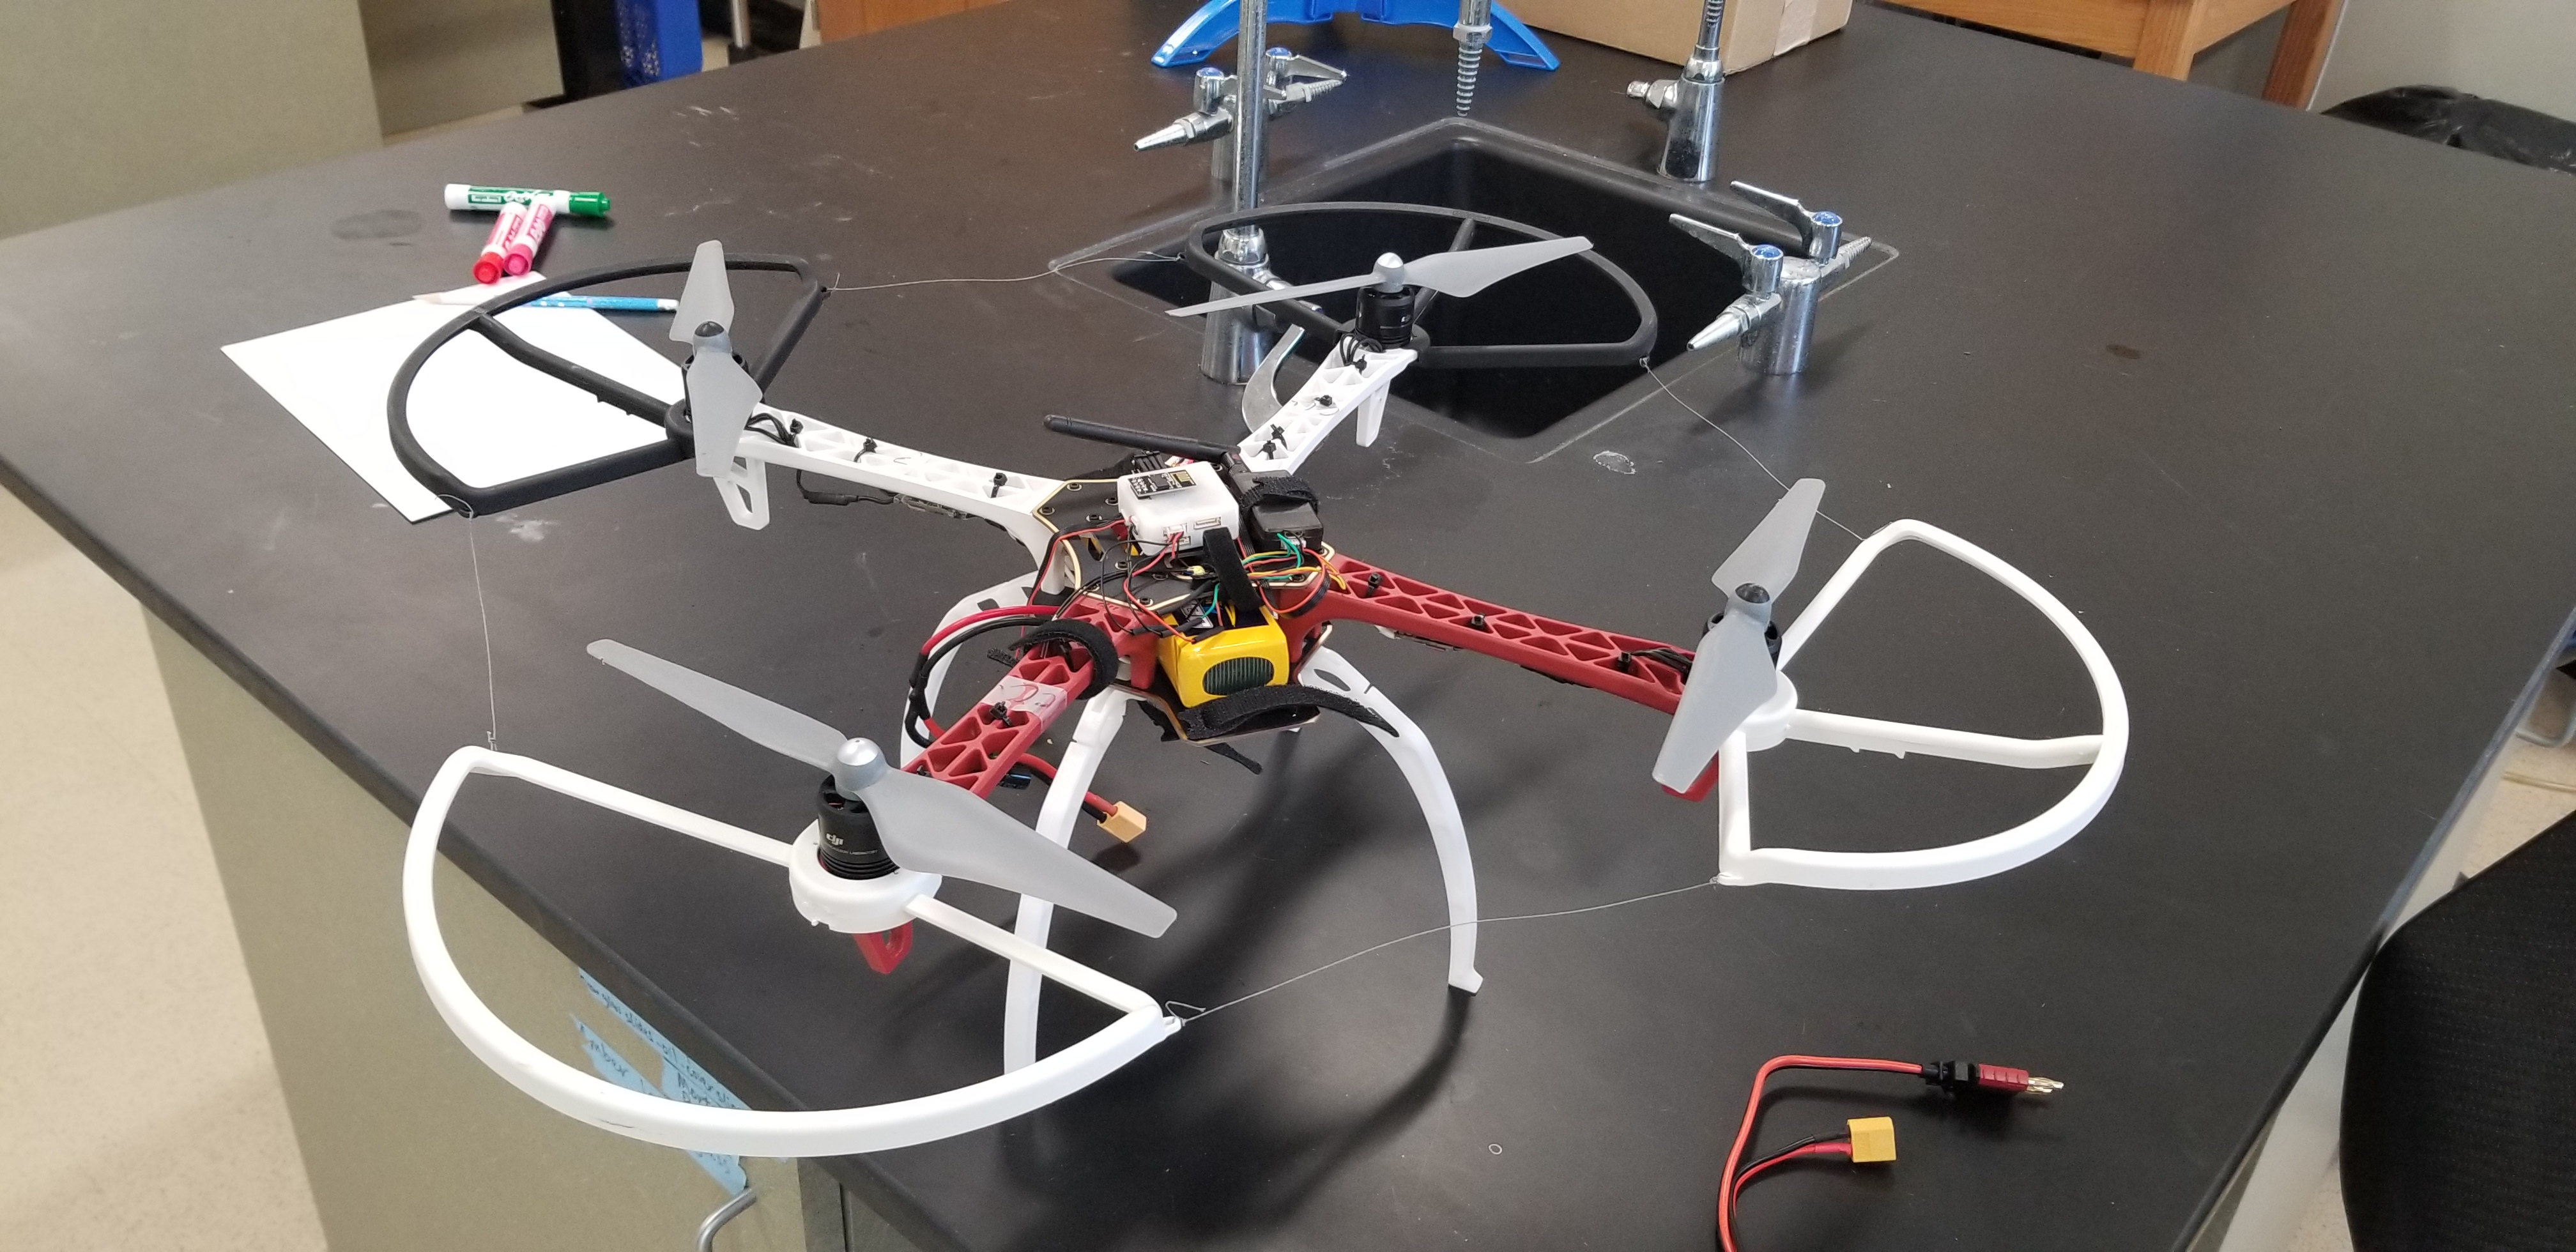
\includegraphics[width=0.5\textwidth]{figs/flamewheel1.jpg}
\caption[Completed airframe]{Completed airframe}
\label{fig:airframe} 
\end{figure}

The Flame Wheel basic airframe is complete, calibrated, tuned, and has made its first few flights, from simple hovers to moving about a large room (Figure: ~\ref{fig:airframe}). We have not set up a practice course yet, but expect to soon.

The build went fairly smoothly. The frame went together without incident. After the main assembly of the airframe, programming and calibration were completed successfully, followed by an attempted first hover. This resulted in an immediate and spectacular crash. After some diagnosis and one more crash (which resulted in damage to one of the propeller guards), it was determined that the ESCs were simply connected to the incorrect ports on the flight controller. Finally, a proper flight test was conducted in which the drone was secured with shock cables to our work bench.

\begin{figure}[!htbp]
\centering 
        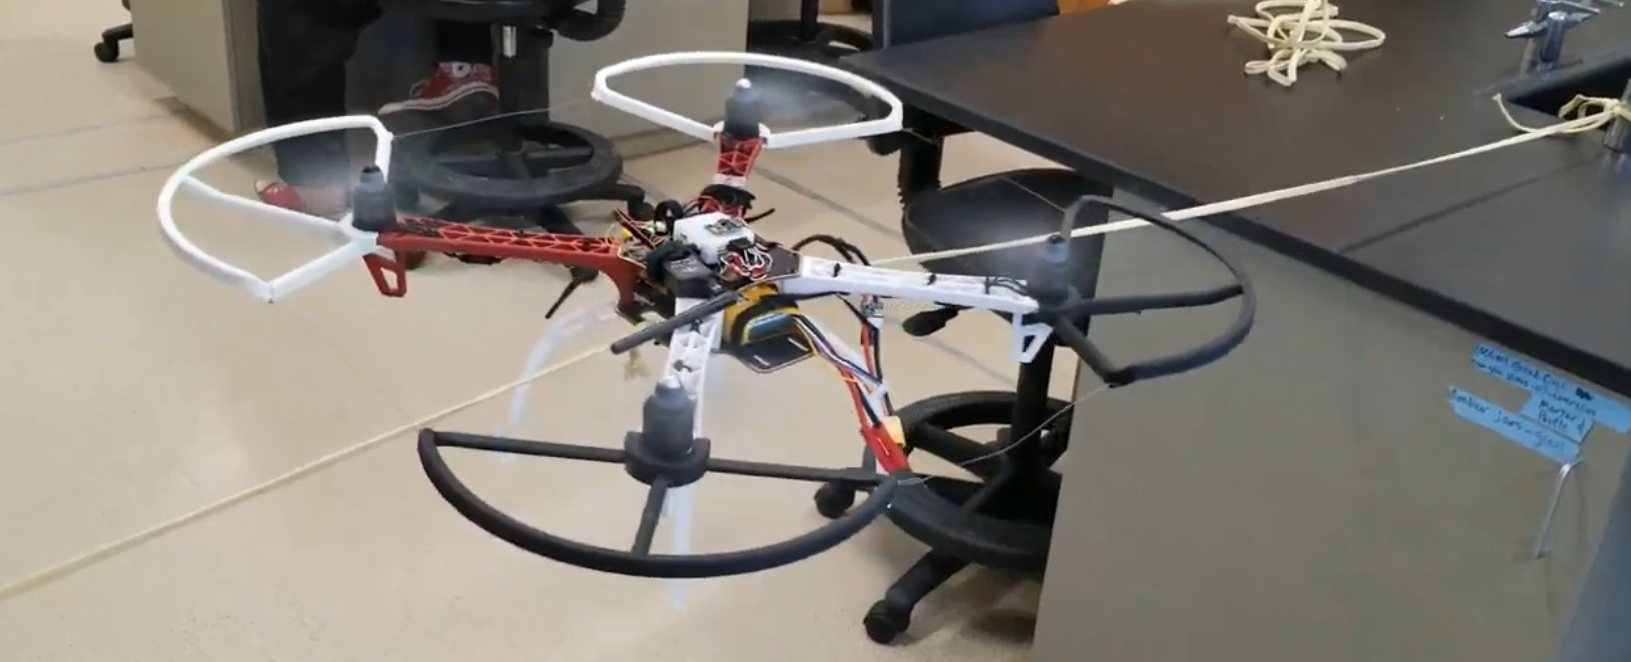
\includegraphics[width=0.5\textwidth]{figs/tune.png}
\caption[Tuning the drone]{Tuning the drone}
\label{fig:tuning} 
\end{figure}

This method of securing the drone to test the PID tuning and ended up being considerably safer and allowed us to be much more confident before attempting a real flight (Figure: ~\ref{fig:tuning}).

As for instrumentation, we are still in the planning and implementation stage. Sensor suite is still a wishlist, and ordering of parts will take place soon.

\section{Progress and Plans for the Challenge}

\begin{figure}[!htbp]
\centering 
        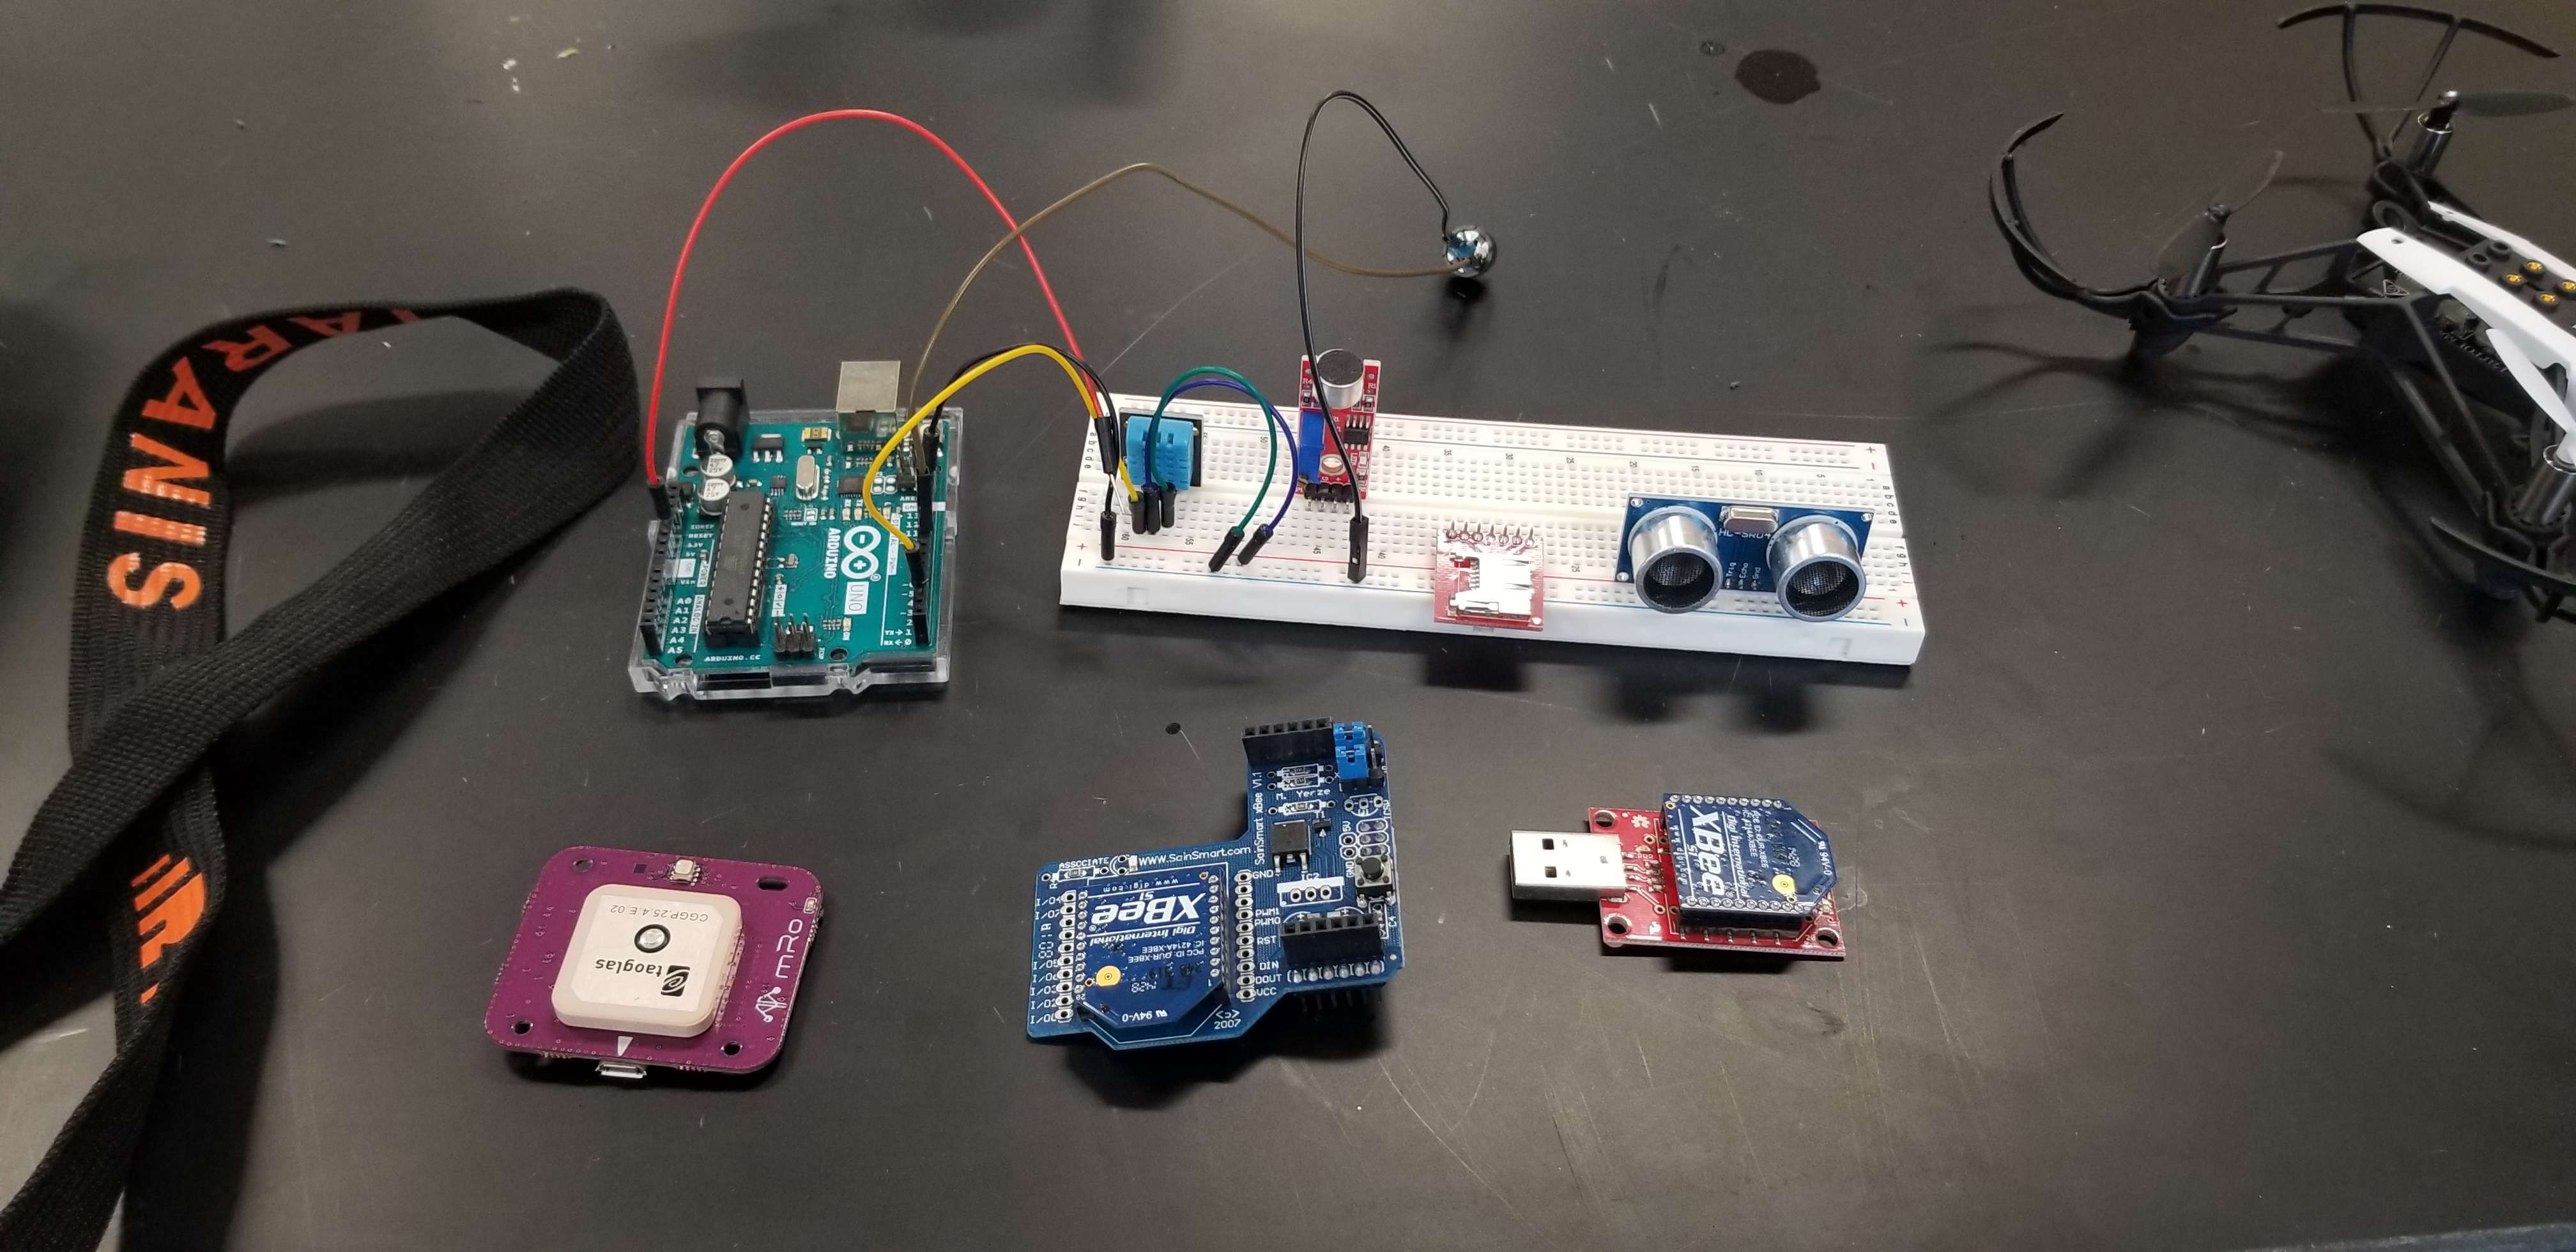
\includegraphics[width=0.5\textwidth]{figs/electronics.jpg}
\caption[Sensor suite and XBee radio]{Sensor suite and XBee radio}
\label{fig:electronics} 
\end{figure}

We have built a few proof-of-concept sensor packages and written code for them. The next step is to order all of the sensors and actuators that we need and to integrate the code for each individual sensor, motor, and communication device. (Figure: ~\ref{fig:electronics})

We will be placing an order for our final sensor suite very soon, and have recruited a student with programming experience which will help to speed up progress on this front.

The plan is to use XBees to transmit all data back to the home base computer in real time.

We would like to, in the end, modularize our instrumentation. If, on competition day, we can swap out instrumentation modules on the fly, we will have a lot of flexibility in handling the sorts of challenges which the course might present.

\section{Plans for Challenge: Flight Day Operations}

We plan to have two or three operators during the flight. To prepare for the flight, we will observe the course and plan a route through it to determine where we want to stop and investigate. The actual operation of the drone will consist of two or three stations. These three stations are:

\begin{itemize}
\item \textbf{Pilot:} Holds the transmitter and pilots the drone. If we have visual on the course, from where the pilot is stationed, they can do some reckoning that way, but there will be a few cameras transmitting video back to a tablet in real time for fine maneuvering.
\item \textbf{Sensors:} Another operator will have access to video feeds and readouts transmitted via XBee from the drone's instrument package. This operator's job will be to record measurements from sensors and keep track of points of interest throughout the course.
\item \textbf{Engineering:} A third operator (it is possible that Engineer and Sensors will be merged into one station) will be in charge of activating any actuators that are built into the drone. This will include various sampling mechanisms (scoops and such) that need to be controlled separately from piloting.
\end{itemize}

\section{Organizational Chart}

Pilot positions are not set in stone. However, this is a reasonable approximation of what the flight team will look like.

\begin{figure}[!htbp]
\centering 
        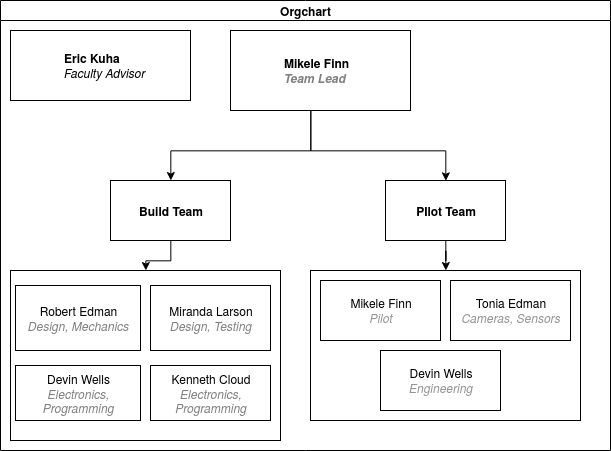
\includegraphics[width=0.5\textwidth]{figs/org_chart.png}
\caption[Organizational Chart]{Organizational Chart}
\label{fig:orgchart} 
\end{figure}

\clearpage

\section{Budget and Parts List}

\begin{table}[!htbp]
\begin{tabular}{lllrrr}
Item                                  & Item Num    & Vendor         & Qty & Cost Per & Total Cost \\
HC-SR04 Ranging Detector              & B004U8TOE6  & Amazon         & 1   & 4.95     & 4.95       \\
USAQ Micro Claw Hook System           & B06VY6R8R9  & Amazon         & 1   & 14.95    & 14.95      \\
Accelerometer/Gyroscope               & B01DK83ZYQ  & Amazon         & 1   & 4.99     & 4.99       \\
HMG MA3D 3 Axis Brushless Gimbal      & 571000061-0 & Hobby King     & 1   & 41.6     & 41.6       \\
Arduino Starter Kit                   & B01CZTLHGE  & Amazon         & 1   & 53.99    & 53.99      \\
Ultimaker 3D 3.00mm Printing Filament & N/A         & Matter Hackers & 1   & 49.95    & 49.95      \\
Hall Effect Sensor                    & 158         & Adafruit       & 1   & 2        & 2          \\
XBee                                  & 968         &                & 2   & 22.95    & 45.9       \\
MLX90640 IR Thermal Camera Breakout   & 4407        & Adafruit       & 1   & 59.95    & 59.95      \\
KNACRO IR Infrared Temperature Sensor & B06WVGD8WJ  & Amazon         & 1   & 12.45    & 12.45      \\
                                      &             &                &     & \textbf{Total}    & \textbf{290.73}    
\end{tabular}
\end{table}

\section{Schedule}

\textbf{11/5/19}    Read books that came with kit, and did research on ideas, and what quadcopters do.

\textbf{11/7/19}    Began laying out pieces and parts for the quadcopter. Took an inventory of parts that came with the kit and got an idea of where everything is supposed to go. Began with soldering wires to home board and screwed the propellers to the framework. We added the motors and connected the wiring. (note no battery is connected yet) Basically pieced together the framework.

\textbf{11/12/19}    Looked over the flight controller, components, and programming. Cut the extra length and finished wiring the motors to the framework. Motors were added, and propeller guards were fitted with R and L and were placed onto the propeller areas. The firmware work began on the flight controller which was a trial and error task. The rest of the time was spent on learning how to configure the controller. Questions came up, and Eric will be contacting the TA's for help. We are having difficulty trying to understand the ground control software, and how it works. Talked about Arduino and learning that part of it. Discussed sending an email out through outlook to every student to reach those that signed up for the quadcopter project.

Finished the day with adding legs onto copter, and guards. Pieces from the guards did snap off but doesn't seem to affect the purpose. We did connect all four legs.

\textbf{11/14/19}    We needed to remove the legs and guards to reconnect the wiring for better position as there was more wire than expected. We needed to tie up any loose wiring. Work continued to configure the controller, and update firmware. Made the decision on which controller would be more useful for the purposes we will be needing.

\textbf{11/19/19}    Finished adjusting the wires around arms of quadcopter. Configured rotation of propellers, so we can move forward with configuring controller. Zip ties were brough in to help rid of any exposed wire. Wires were wrapped around the arms and zip ties were used to hold into place. Continuation of connecting flight controller and updating firmware. Configured Ground Control, and configured flight controller. Thoughts of how to connect GPS and how. What are we going to use to place the GPS at the furthest point away from the battery? Ideas of utilizing 3D printing.

\textbf{11/21/19}    Battery was connected and tested. Rotation of motors were not sound and could tell there was an issue. Test was completed on rotation of motors, to check if placed in the right areas. Motors were adjusted and were rotating in the correct directions from one another. Battery was unplugged and proceeded with adding the propellers to the motors. Watched a few videos on how to adjust the trim or stabilizing the quadcopter. Idea from U of M was to have someone hold a string tied to the quad so adjustments could be made.

\textbf{12/3/19}    Table edges and disks were used to stabilize quadcopter so adjustments could be made. Video was taken of this portion, and shared with other team members that were not able to make it. Big step in getting the quadcopter ready for flight. Brainstorming session on what inventory we are going to need additionally. Where the funding will come from. What is going to be our barriers, and what we think we definitely need to add to the quadcopter.

\textbf{12/10/19}    Quadcopter was tested for flight. A small piece had broken off the propeller guard, which will not affect it's flight what so ever. Discussions began of temperature control, grappling hook, scoop, and dropper, etc. What challenges will there be? When the report is due, and what else is needed to continue practice. Some students agreed to work on flying the drone, others agreed to be more mechanical behind the scenes. Which cameras will be used? Which workstation are we going to use, what type? Etc.

Future Schedule

January 2020: Finalize team and begin designing and implementing electronic components.

February 2020: 3D print housings and other components that require fabrication. Practice Flying.

March 2020: Practice flying the drone and drill possible scenarios for the challenge.

%\section{References}

\nocite{*}

\bibliographystyle{acm}
\bibliography{bib/references}

%\bibliographystyle{plainnat}
%\bibliography{bib/sample.bib} % The file containing the bibliography

%----------------------------------------------------------------------------------------


\end{document}
